%
% 00_Einleitung.tex
%
% (c) 2020 Prof Dr Andreas Müller, Hochschule Rapperswil
%
% !TEX root = ../../buch.tex
% !TEX encoding = UTF-8
%
\section{Einleitung\label{jpeg:section:einleitung}}
\rhead{Einleitung}
\begin{figure}
    \centering
    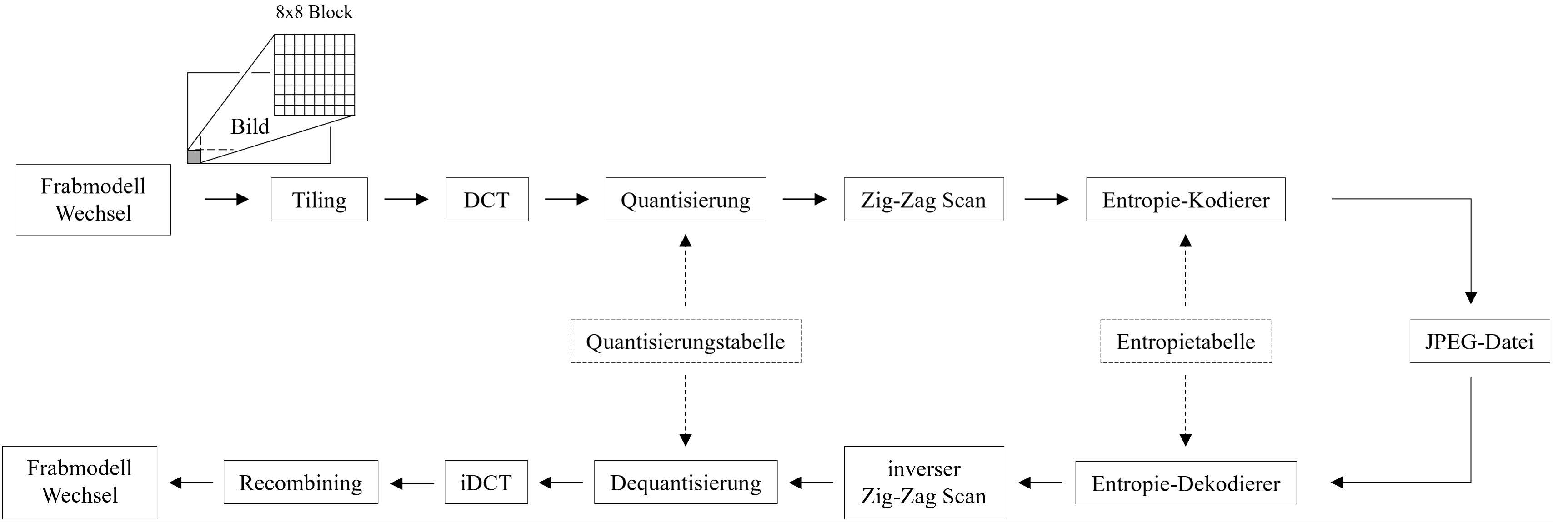
\includegraphics[width=\linewidth]{papers/jpeg/pictures/kompressionsschema.pdf}
    \caption{Vorgehen bei der Kompression und Dekompression von JPEG
        \label{jpeg:fig:kompressionsschema}}
\end{figure}
Daten können besonders effizient übertragen oder gespeichert werden, wenn sie zuerst komprimiert werden.
Das kann in vollständig rekonstruierbarer Form oder mit Verlusten geschehen.

Verlustloses Komprimieren gelingt, indem man einen Kodieralgorithmus auf die Daten anwendet und die redundanten Informationen wie in einem Wörterbuch speichert und jeweils darauf referenziert. Beim verlustbehafteten Verfahren werden z.B. bei Bildern die Daten entfernt, die für Menschen nicht sichtbar sind, um den Inhalt zu reduzieren.

Es gibt inzwischen einige Methoden um Bilder zu komprimieren.
In diesem Kapitel soll es um die beiden Algorithmen von der Joint Photographic Experts Group (JPEG) gehen.


Bilder werden zuerst mit einer Vorverarbeitung auf die Transformation vorbereitet.
Das sind Farb\-raumtransformationen und Einteilung in kleinere Bereiche, dieser Schritt heisst Tiling.
Anschliessend wird die Basistransformation durchgeführt und die Koeffizienten mit einer Tabelle quantisiert und ganzzahlig gerundet.
Die aus der Quantisierung entstandenen Werte werden entropiekodiert, meistens wird das Prinzip von Huffman verwendet.
Die verwendete Methode wird im File abgelegt.
Zudem werden die Tabellen der unterschiedlichen Quantisierungen und Kodierungen mit abgespeichert (s. Abb. \ref{jpeg:fig:kompressionsschema}).
Für die Dekompression werden diese Schritte rückwärts angewandt, wobei die verloren gegangenen Informationen bei der Quantisierung nicht wieder hergestellt werden können. 

Grundlegend werden die Bilder mithilfe von verschiedenen Methoden in Basisfunktionen aufgeteilt, zu denen jeweils die Koeffizienten berechnet werden.
Damit ist es möglich, diese in einem späteren Schritt zu manipulieren und Daten einzusparen. 
Bei JPEG ist das die discrete cosine transform (DCT) und bei JPEG-2000 die discrete wavelet transform (DWT).

Das Kapitel basiert auf Inhalte des Papers \textit{Bilddatenkompression mit JPEG und JPEG2000} \cite{jpeg:laurahochstrat}